\documentclass[a4paper]{scrartcl}
\usepackage[utf8]{inputenc}
\usepackage[english]{babel}
\usepackage{graphicx}
\usepackage{lastpage}
\usepackage{pgf}
\usepackage{wrapfig}
\usepackage{fancyvrb}
\usepackage{fancyhdr}
\usepackage{float}
\usepackage{hyperref}
\usepackage{amssymb}% http://ctan.org/pkg/amssymb
\usepackage{pifont}% http://ctan.org/pkg/pifont
\newcommand{\cmark}{\ding{51}}%
\newcommand{\xmark}{\ding{55}}%
\pagestyle{fancy}

% Create header and footer
\headheight 27pt
\pagestyle{fancyplain}
\lhead{\footnotesize{Internet Applications, ID1354}}
\chead{\footnotesize{Name of the Report}}
\rhead{}
\lfoot{}
\cfoot{\thepage\ (\pageref{LastPage})}
\rfoot{}

% Create title page
\title{Laravel or How To Get Lost In Documentation}
\subtitle{Internet Applications, ID1354}
\author{Linus Berg Linus@Fenix.me.uk}
\date{\today}

\begin{document}

\maketitle

\section{Introduction}

\noindent
The task of this seminar was to move the initially unstructured PHP files to a MVC structure,
such as the Laravel framework (my choice).
\noindent
\\\\
On top of that the security should be improved to further accomodate a production server / code,
passwords should be hashed et cetera, along with other security concerns.


\section{Literature Study}
The majority of this seminar was spent trying to learn Laravel, all of the learning was done
on their official documentation.\\
\href{https://laravel.com/docs/5.7}{Laravel Docs}


\section{Method}

The first objective was to select which framework to use, the framework chosen was
Laravel for the overwhelming amount of support / documentation available, it is the most
widespread PHP framework currently, so it seemed like a good choice.
\\\\
\noindent
Once the PHP framework was chosen the conversion of the code started, firstly
by setting up the routing, then the controllers, and if needed models. Each step
included reading the documentation, for example, during the route creation, I went
back and forth between implementation and reading the documentation for routes.
\\\\
\noindent
For each route that was setup the according view was also created using the
Laravel Blade templating system. In each view that required AJAX request, the
corresponding Ajax requests were also implemented in the routes and setup in the
controller. It resulted in a lot of back and forth between different files,
however it turned out good enough in the end. 
\\\\
\noindent
Because templates were already utilised in seminar one, it was merely a matter
of changing them from the Jinja templating engine syntax to the Laravel one, which
was extremely easy.
\\\\
The security concerns were almost an afterthought as Laravel handles a lot of
it for you by default.
\begin{center}
    \begin{tabular}{  l | r }
    Tool & Choice \\ 
    \hline
    Editor & \textit{Vim}\\
    Version Control & \textit{Git - Github}\\
    Web Server & \textit{nginx}\\
    Database & \textit{PostgreSQL 10.5-1}\\
    PHP & \textit{7.2.10-1} \\
    Framework & \textit{Laravel 5.7}\\
    UML Editor & \textit{Dia}\\
    \end{tabular}
\end{center}
\section{Result}
\href{https://github.com/linus-dev/KTH-Projects/tree/master/ID1354/3/laravel}
{Github}
\subsection{Framework \& code}
When porting the code to Laravel, the framework makes several abstraction layers of code,
for example, routing is a simple call to \textit{Route::Get()}, this leads to significantly less
code in the final result.
\\\\
\noindent
As such, the final class diagram is below, with each of the routing calls to a controller,
the routes \textit{/comment/post/} and \textit{/comment/delete} are authenticated by the
\textbf{auth} middleware. The class diagram is quite small due to the abstractions that laravel makes.

\begin{figure}[H]
  \begin{center}
    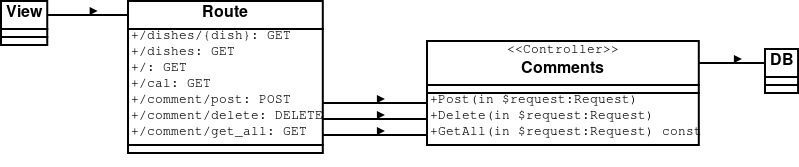
\includegraphics[scale=0.5]{images/class.png}
    \caption{Laravel class diagram.}
    \label{fig:class_diagram}
  \end{center}
\end{figure}

\begin{figure}[H]
  \begin{center}
    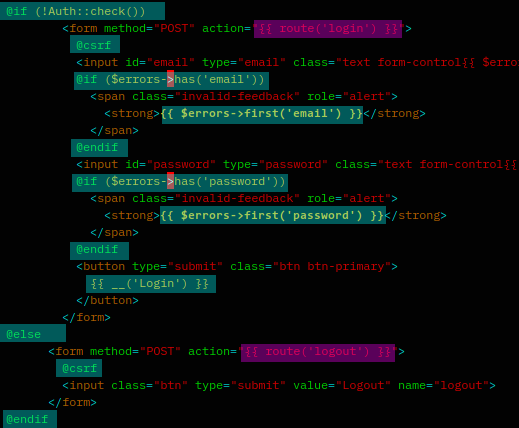
\includegraphics[scale=1.0]{images/blade.png}
    \caption{Laravel blade template.}
    \label{fig:blade}
  \end{center}
\end{figure}

\noindent
In \ref{fig:blade} a Laravel blade example is shown where the Laravel commands
are highlighted. Laravel handles all authentication needs and therefor
a lot of code does not need to be written to deal with the user logging in / commenting.

\begin{figure}[H]
  \begin{center}
    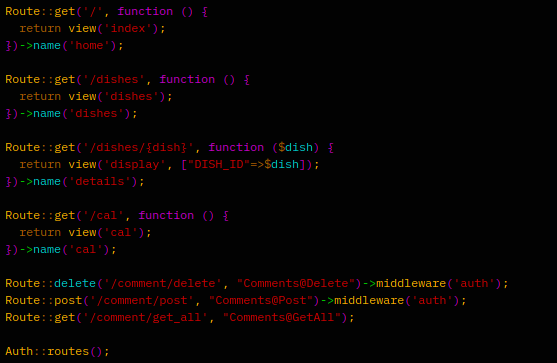
\includegraphics[scale=1.0]{images/routes.png}
    \caption{Laravel routing.}
    \label{fig:routes}
  \end{center}
\end{figure}

\noindent
The routing in laravel is extremely simple, in \ref{fig:routes} the entirety of the
routing used for the recipes website is shown, as described earlier, the \textit{delete} and
\textit{post} are authenticated using the auth module from Laravel.
Each of the \textit{/comment/} API is called by using Ajax in the webpage,
which made it a lot easier to port the code from the standalone structure to 
the Laravel framework. Other than that, most of the functionality of Laravel is
abstracted into simpler methods and not exposed to the user.

\begin{figure}[H]
  \begin{center}
    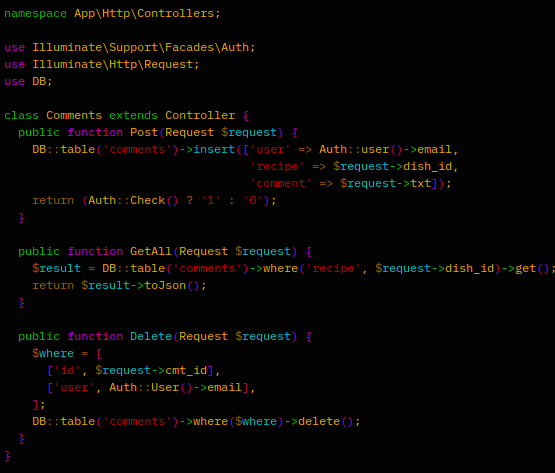
\includegraphics[scale=1.0]{images/db.png}
    \caption{Comments controller.}
    \label{fig:comments}
  \end{center}
\end{figure}
\noindent
The controller shown in \ref{fig:comments} is the only functionality (other than routes)
that Laravel utilises, that was written specifically for this site, the simple returns
could be further improved to contain more information. Each method simply manipulates or
gathers data from the database layer, and it utilises the Laravel query builder,
unforunately this functionality is also abstracted.
\newpage
\subsection{Security}
\begin{itemize}
\item{File System Security \checkmark}
\item{Input filtering \checkmark}
\item{Database security \checkmark}
\item{Password Encryption \checkmark}
\item{XSS \checkmark}
\item{Impersonation \checkmark}
\item{HTTPS \xmark}
\end{itemize}
Above are the security concerns that should be considered/implemented,
the implemented ones are marked with a checkmark.
As stated earlier the security concerns were mostly an after thought as Laravel
handles many of them, for example, Laravel handles, \textit{Input filtering,
Password encryption, and Impersionation}, however, it also handles a lot more in
the background that the user is not exposed to. Impersonation is handled via
CSRF tokens which are also sent in the header of each Ajax request.
\\\\
\noindent
I utilise Arch Linux on my personal laptop and CentOS with SELINUX
on my rackserver at home, so I am no stranger to setting up the user permissions
in the file system, the nginx user was always set up to minimize the amount
of access it has. The database was correctly setup as well with the user, and
all remote access was promptly removed.
\\\\
\noindent
As for the remaining two check marks (\textit{XSS \& HTTPS}), XSS should not be
possible due to the input filtering occuring by Laravel.
I did not setup HTTPS on my local test server, however obviously these days HTTPS
should be used by any website to secure the connection between user and server.
I do however run HTTPS on my personal website
\href{Https://themountain.xyz}{Https://TheMountain.XYZ} as an example of how I 
utilise HTTPS.
\section{Discussion}

During this seminar I chose Laravel because of the simplicty of the framework,
however as stated many times in the text, it has a lot of abstraction layers,
and that leads to less understanding of making a PHP MVC structure, however, it
is rare these days to develop your own framework and not modify an existing one.
\\\\
\noindent
I used a database in the previous seminars and therefor I used one in this one as
well since it integrates very easily into Laravel, but it also lead to optional
task 2 being solved without even trying.
\end{document}
